%me=0 student solutions (ps file), me=1 - my solutions (sol file), me=2 - assignment (hw file)
\def\me{0}
\def\num{1}  %homework number
\def\due{Sunday, October 11}  %due date
\def\course{CSCI-GA.2110.001 Programming Languages} %course name, changed only once
\def\name{GOWTHAM GOLI (N17656180)}   %student changes (instructor keeps!)
%
\iffalse
INSTRUCTIONS: replace # by the homework number.
(if this is not ps#.tex, use the right file name)

  Clip out the ********* INSERT HERE ********* bits below and insert
appropriate TeX code.  Once you are done with your file, run

  ``latex ps#.tex''

from a UNIX prompt.  If your LaTeX code is clean, the latex will exit
back to a prompt.  To see intermediate results, type

  ``xdvi ps#.dvi'' (from UNIX prompt)
  ``yap ps#.dvi'' (if using MikTex in Windows)

after compilation. Once you are done, run

  ``dvips ps#.dvi''

which should print your file to the nearest printer.  There will be
residual files called ps#.log, ps#.aux, and ps#.dvi.  All these can be
deleted, but do not delete ps1.tex. To generate postscript file ps#.ps,
run

  ``dvips -o ps#.ps ps#.dvi''

I assume you know how to print .ps files (``lpr -Pprinter ps#.ps'')
\fi
%
\documentclass[11pt]{article}
\usepackage{amsfonts}
\usepackage{latexsym}
\usepackage{listings}
\usepackage{amsmath}
\usepackage{float}
\usepackage{epsfig}
\setlength{\oddsidemargin}{.0in}
\setlength{\evensidemargin}{.0in}
\setlength{\textwidth}{6.5in}
\setlength{\topmargin}{-0.4in}
\setlength{\textheight}{8.5in}

\newcommand{\handout}[5]{
   \renewcommand{\thepage}{#1, Page \arabic{page}}
   \noindent
   \begin{center}
   \framebox{
      \vbox{
    \hbox to 5.78in { {\bf \course} \hfill #2 }
       \vspace{4mm}
       \hbox to 5.78in { {\Large \hfill #5  \hfill} }
       \vspace{2mm}
       \hbox to 5.78in { {\it #3 \hfill #4} }
      }
   }
   \end{center}
   \vspace*{4mm}
}

\newcounter{pppp}
\newcommand{\prob}{\arabic{pppp}}  %problem number
\newcommand{\increase}{\addtocounter{pppp}{1}}  %problem number

%first argument desription, second number of points
\newcommand{\newproblem}[2]{
\ifnum\me=0
\ifnum\prob>0 \newpage \fi
\increase
\setcounter{page}{1}
\handout{\name, Homework \num, Problem \arabic{pppp}}{\today}{Name: \name}{Due:
\due}{Solutions to Problem \prob\ of Homework \num\ (#2)}
\else
\increase
\section*{Problem \num-\prob~(#1) \hfill {#2}}
\fi
}

%\newcommand{\newproblem}[2]{\increase
%\section*{Problem \num-\prob~(#1) \hfill {#2}}
%}

\def\squarebox#1{\hbox to #1{\hfill\vbox to #1{\vfill}}}
\def\qed{\hspace*{\fill}
        \vbox{\hrule\hbox{\vrule\squarebox{.667em}\vrule}\hrule}}
\newenvironment{solution}{\begin{trivlist}\item[]{\bf Solution:}}
                      {\qed \end{trivlist}}
\newenvironment{solsketch}{\begin{trivlist}\item[]{\bf Solution Sketch:}}
                      {\qed \end{trivlist}}
\newenvironment{code}{\begin{tabbing}
12345\=12345\=12345\=12345\=12345\=12345\=12345\=12345\= \kill }
{\end{tabbing}}

%\newcommand{\eqref}[1]{Equation~(\ref{eq:#1})}

\newcommand{\hint}[1]{({\bf Hint}: {#1})}
%Put more macros here, as needed.
\newcommand{\room}{\medskip\ni}
\newcommand{\brak}[1]{\langle #1 \rangle}
\newcommand{\bit}[1]{\{0,1\}^{#1}}
\newcommand{\zo}{\{0,1\}}
\newcommand{\C}{{\cal C}}

\newcommand{\nin}{\not\in}
\newcommand{\set}[1]{\{#1\}}
\renewcommand{\ni}{\noindent}
\renewcommand{\gets}{\leftarrow}
\renewcommand{\to}{\rightarrow}
\newcommand{\assign}{:=}

\newcommand{\AND}{\wedge}
\newcommand{\OR}{\vee}

\newcommand{\For}{\mbox{\bf For }}
\newcommand{\To}{\mbox{\bf to }}
\newcommand{\Do}{\mbox{\bf Do }}
\newcommand{\If}{\mbox{\bf If }}
\newcommand{\Then}{\mbox{\bf Then }}
\newcommand{\Else}{\mbox{\bf Else }}
\newcommand{\While}{\mbox{\bf While }}
\newcommand{\Repeat}{\mbox{\bf Repeat }}
\newcommand{\Until}{\mbox{\bf Until }}
\newcommand{\Return}{\mbox{\bf Return }}
\newcommand{\Swap}{\mbox{\bf Swap }}

\lstset{language=Ada}

\begin{document}

\ifnum\me=0
%\handout{PS\num}{\today}{Name: **** INSERT YOU NAME HERE ****}{Due:
%\due}{Solutions to Problem Set \num}
%
%I collaborated with *********** INSERT COLLABORATORS HERE (INDICATING
%SPECIFIC PROBLEMS) *************.
\fi
\ifnum\me=1
\handout{PS\num}{\today}{Name: Yevgeniy Dodis}{Due: \due}{Solution
{\em Sketches} to Problem Set \num}
\fi
\ifnum\me=2
\handout{PS\num}{\today}{Lecturer: Yevgeniy Dodis}{Due: \due}{Problem
Set \num}
\fi


\newproblem{Insertion Sort Using a Linked List}{}

Provide regular expressions for defining the syntax of the following.

\begin{itemize}

\item[(a)]Passwords consisting of letters and digits that contain at least two upper case letters
and one digit. They can be of any length (obviously at least three characters).

\ifnum\me<2
\begin{solution}
\begin{alignat*}{3}
& Letter &&\rightarrow && UC|LC\\
& UC &&\rightarrow && [A-Z]\\
& LC &&\rightarrow && [a-z]\\
& Digit &&\rightarrow && [0-9]\\
& Password &&\rightarrow && (Letter \cup Digit)^* Digit.UC (Letter \cup Digit)^* UC (Letter \cup Digit)^*\\
& && && |(Letter \cup Digit)^* UC.Digit (Letter \cup Digit)^* UC (Letter \cup Digit)^*\\
& && && |(Letter \cup Digit)^* UC (Letter \cup Digit)^* UC.Digit (Letter \cup Digit)^*\\
\end{alignat*}
\end{solution}
\fi

\item[(b)] Floating point literals that specify an exponent, such as the following: $2.43876E13$ (representing $243.867 \times 10^{13}$
).

\ifnum\me<2
\begin{solution}
Assuming that the (E) part can be optional,
The left side of the exponent (E) part can take the following forms
\begin{itemize}
\item Left side of the decimal point is 0, Right side of the decimal point allows one or more digits from 0-9. Therefore, regular expression is $0.[0-9]+$
\item Left side of decimal point is empty, Right side of the decimal point allows one or more digits from 0-9 . Therefore, regular expression is $.[0-9]+$
\item There is no decimal point. Regular expression is $[1-9][0-9]^*$
\item The left side of the decimal starts with 1-9 followed by zero or more digits from 0-9. The right side of the decimal allows one or more digits from 0-9. Therefore, regular expression is $[1-9][0-9]^*.[0-9]+$
\end{itemize}
(Note that ? makes the preceding token optional and + makes the token appear at least once)
Therefore the final regular expression is

\centering{
(($0?.[0-9]+)|([1-9][0-9]^*)|([1-9][0-9]^*.[0-9]+$)) $(E [0-9]+)?$
}

\end{solution}
\fi

\item[(c)] Procedure names that: must start with a letter; may contain letters, digits, and (underscore); and must be no more than 10 characters.

\ifnum\me<2
\begin{solution}
\begin{alignat*}{3}
& Letter    &\rightarrow & [A-Z]|[a-z] \\
& Digit     &\rightarrow & [0-9]\\
& Procedure &\rightarrow & Letter. \underbrace{(\epsilon \cup Letter \cup \_ \cup Digit ) \ldots (\epsilon \cup Letter  \cup \_ \cup Digit )}_\text{9 times}\\
\end{alignat*}
\end{solution}
\fi

\end{itemize}


\newproblem{Multiplying Binary Integers}


\begin{itemize}

\item[(a)]Provide a simple context-free grammar for the language in which the following program is
written. You can assume that the syntax of names and numbers are already defined using
regular expressions (i.e. you don’t have to define the syntax for names and numbers)

\begin{lstlisting}

program one;
  var x;
  
  function f(var x, var y)
  var z;
  begin
  z := x+y-1;
  return z*2;
  end f;
  
  procedure g()
  var a;
  begin
  a := 3;
  x := a;
  end g;
  	
begin
g();
print(f(x));
end one;
\end{lstlisting}

\ifnum\me<2
\begin{solution}
\begin{alignat*}{3}
&<Program>     &\rightarrow \,\,\,& program <prog\_name> ; \,\,\,  <prog\_decl>\\
& & & \,\, begin <body> end <prog\_name>;\\
&<prog\_decl>  &\rightarrow \,\,\,&  <var\_decl>\,\,\, <func\&proc\_decl>\\
&<var\_decl>   &\rightarrow \,\,\, &  \epsilon \,\, |\,\,  var <identifier> ; \,\,\, <var\_decl>\\
&<func\&proc\_decl> &\rightarrow \,\,\ & \epsilon \,\,\, | <func\_decl>\,\,\,<func\&proc\_decl>\\
& & &\,\, | \,\, <proc\_decl>\,\,\,<func\&proc\_decl>\\
&<func\_decl> &\rightarrow \,\,\ &  function <func\_name> (<param>)\,\, <var\_decl> \\
& & &\,\, begin  <body>  end <func\_name>; \\
&<proc\_decl>  &\rightarrow \,\,\ &  procedure <proc\_name> (<param>) \,\, <var\_decl>\\
& & &\,\,begin <body> end <proc\_name>;\\
&<body>        &\rightarrow  \,\,\ & <stmt\_list>\\
&<stmt\_list>  &\rightarrow \,\,\ &  \epsilon \,\,\, | null; \,\, | <stmt>; \,\,\,<stmt\_list>\\
&<stmt>        &\rightarrow \,\,\ & \epsilon \,\,\, | <identifier> := <expr> \,\,\, | \,\,\, return <expr> \,\,\, \\& & & \,\,\,| \,\, <func\_name> (<args>) \,\,\,| \,\,\, <proc\_name>(<args>)\\
&<param>       &\rightarrow \,\,\, &  \epsilon \,\,\,| var <identifier> | \,\,\, function <func\_name> |\,\,\,  procedure <proc\_name>\\
& & &| \,\,\,var <identifier>, <param> \,\,\, | \,\,\, function <func\_name>, <param>\\ & & & | \,\,\,  procedure <proc\_name>, <param>\\
&<args>        &\rightarrow \,\,\, &  \epsilon \,\,\, | \,\,\, <identifier> \,\,\,
| \,\,\, <func\_name> (<args>)\,\,\, |  <proc\_name> (<args>)\\ & & &| \,\,\, <identifier>, <args>  \,\,\,| <func\_name> (<args>) , <args> \\ & & & | \,\,\, <proc\_name> (<args>) ,<args>\\
&<expr>        &\rightarrow \,\,\, & <expr> + <expr> \,\, | \,\, <expr> - <expr> \,\, | \,\, <expr> * <expr>\\
& & & \,\, | \,\, <expr>/<expr> \,\, | \,\, (<expr>) \,\, | \,\, number \,\, | \,\, identifier\\
&<prog\_name>   &\rightarrow \,\,\, & identifier\\
&<proc\_name>   &\rightarrow \,\,\, & identifier\\
&<func\_name>   &\rightarrow \,\,\, & identifier\\
\end{alignat*}
\end{solution}
\fi
\pagebreak
\item[(b)]Draw the parse tree for the above program

\ifnum\me<2
\begin{solution}
\begin{figure}[H]
	\centering
	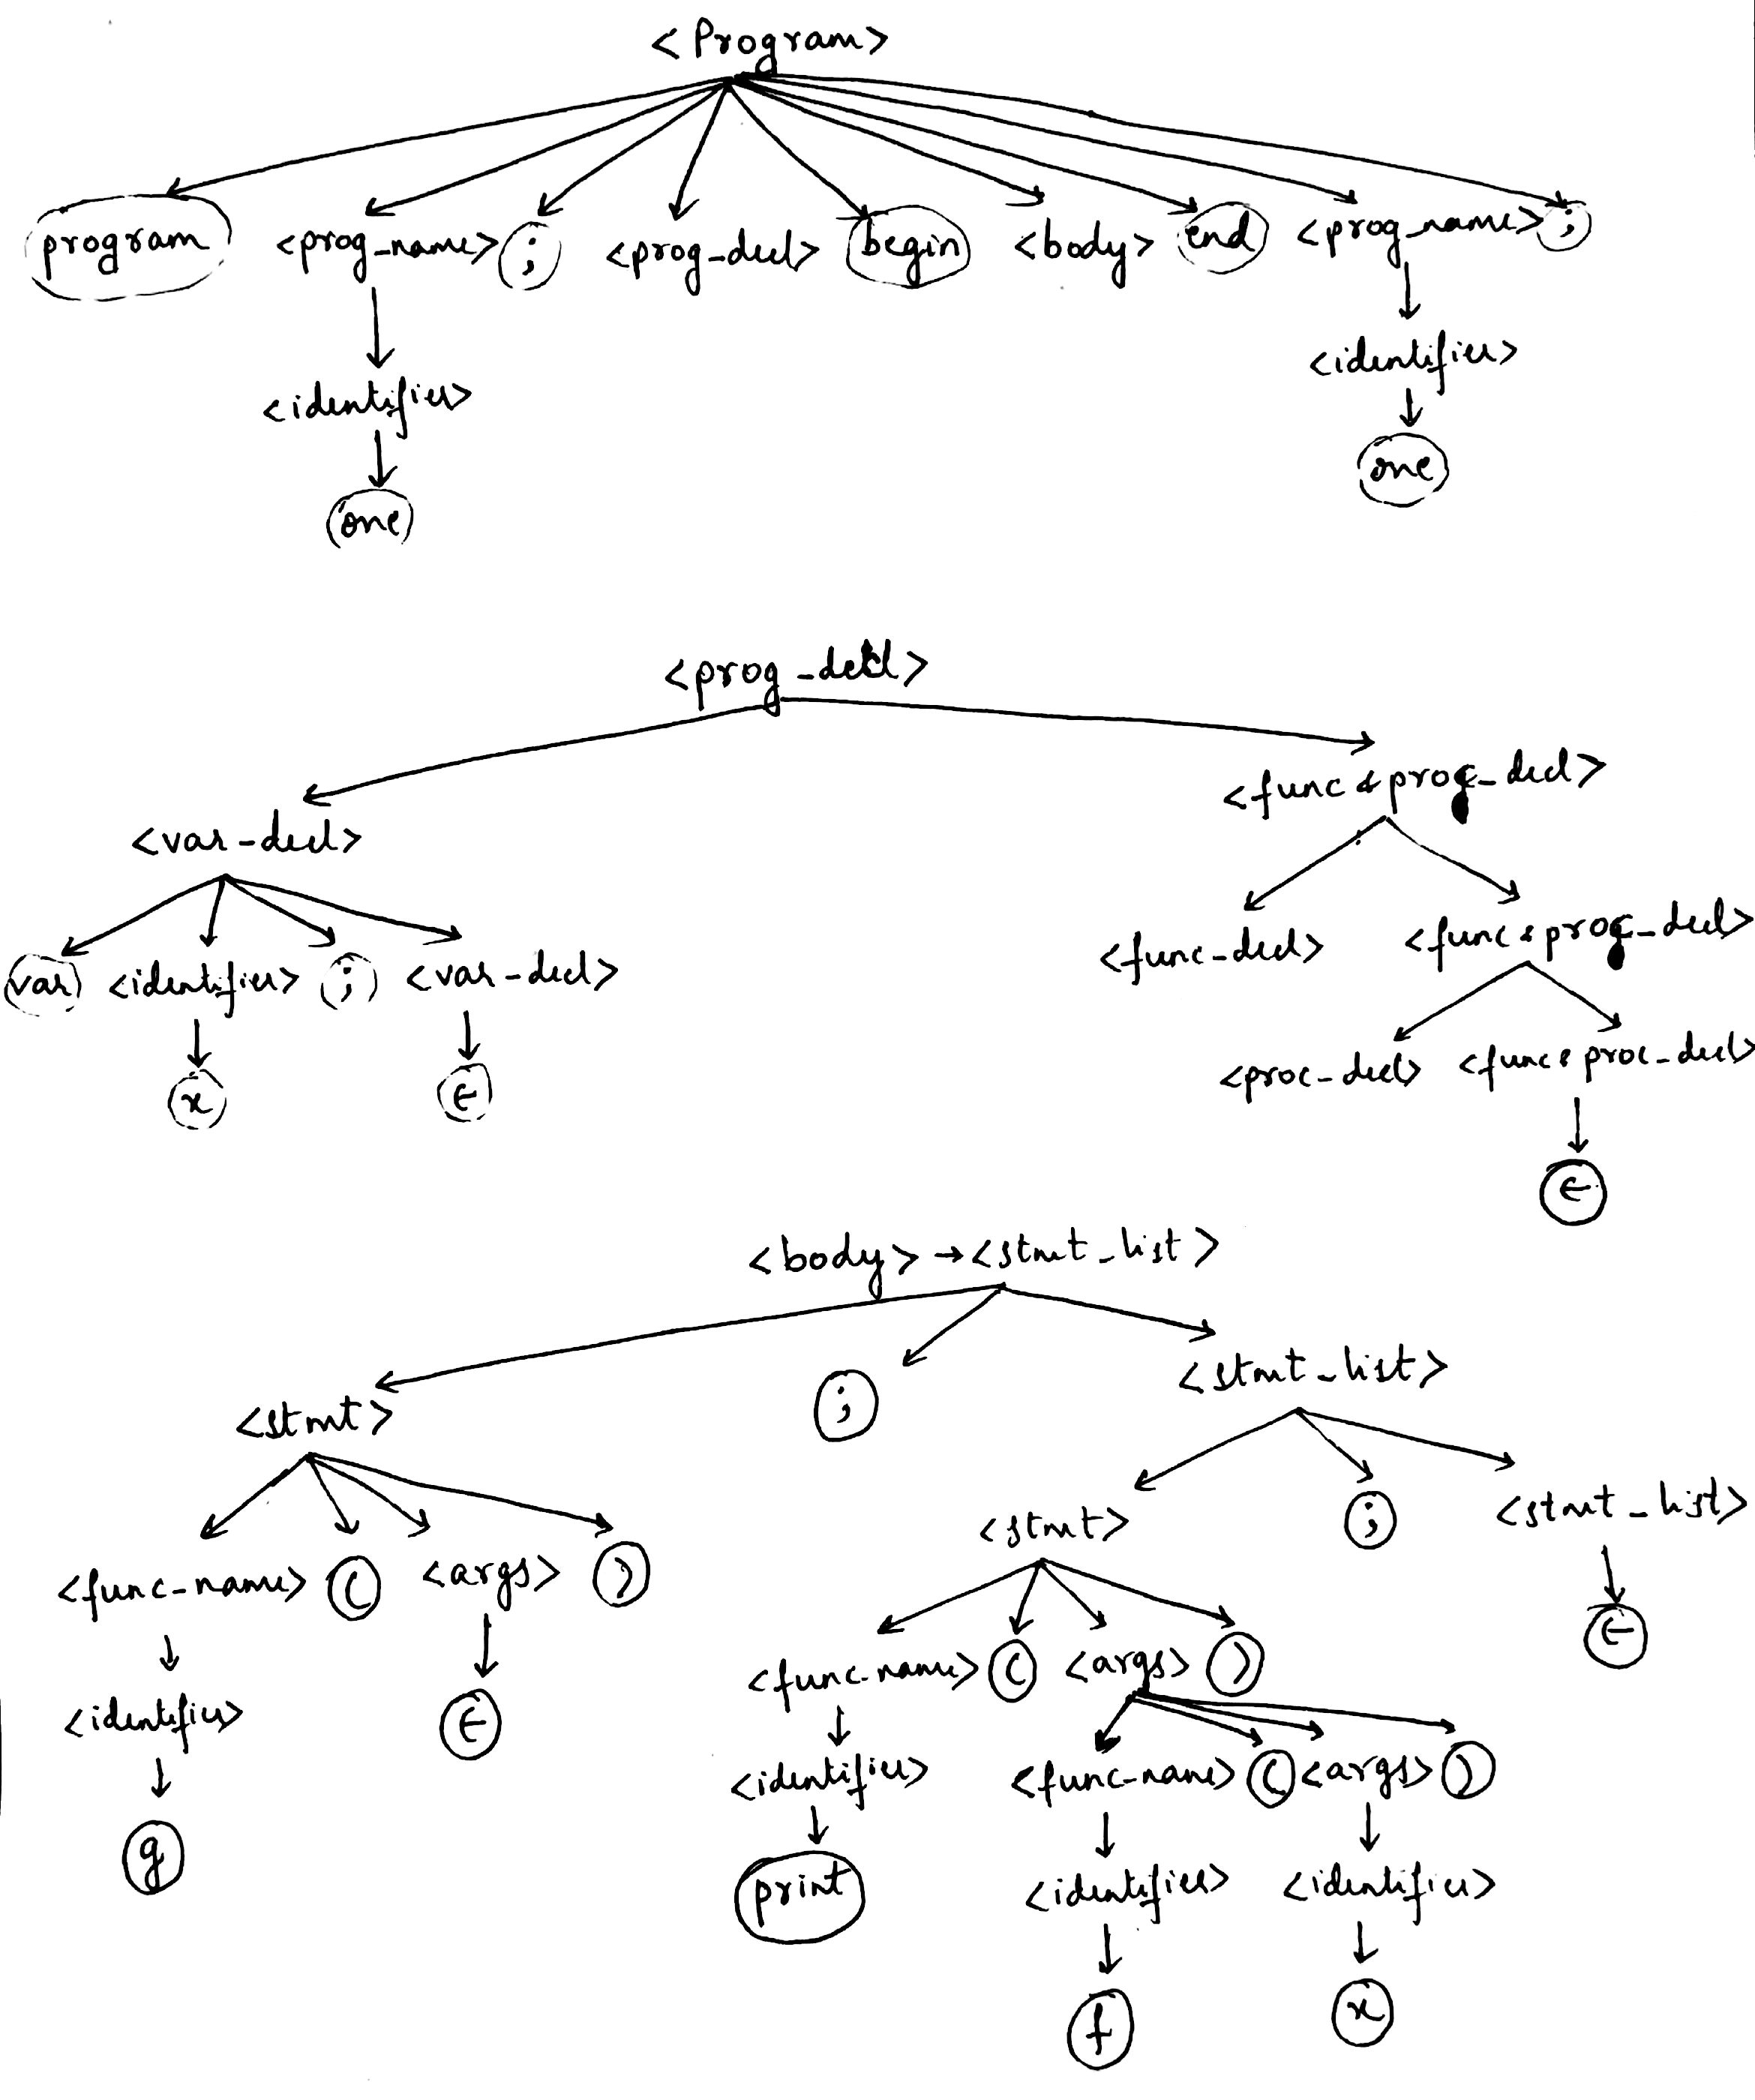
\includegraphics[width=0.95\columnwidth]{one.jpg}
	\caption{Parse tree of Program \textit{one}}
	\label{1}
\end{figure}


\begin{figure}[H]
	\centering
	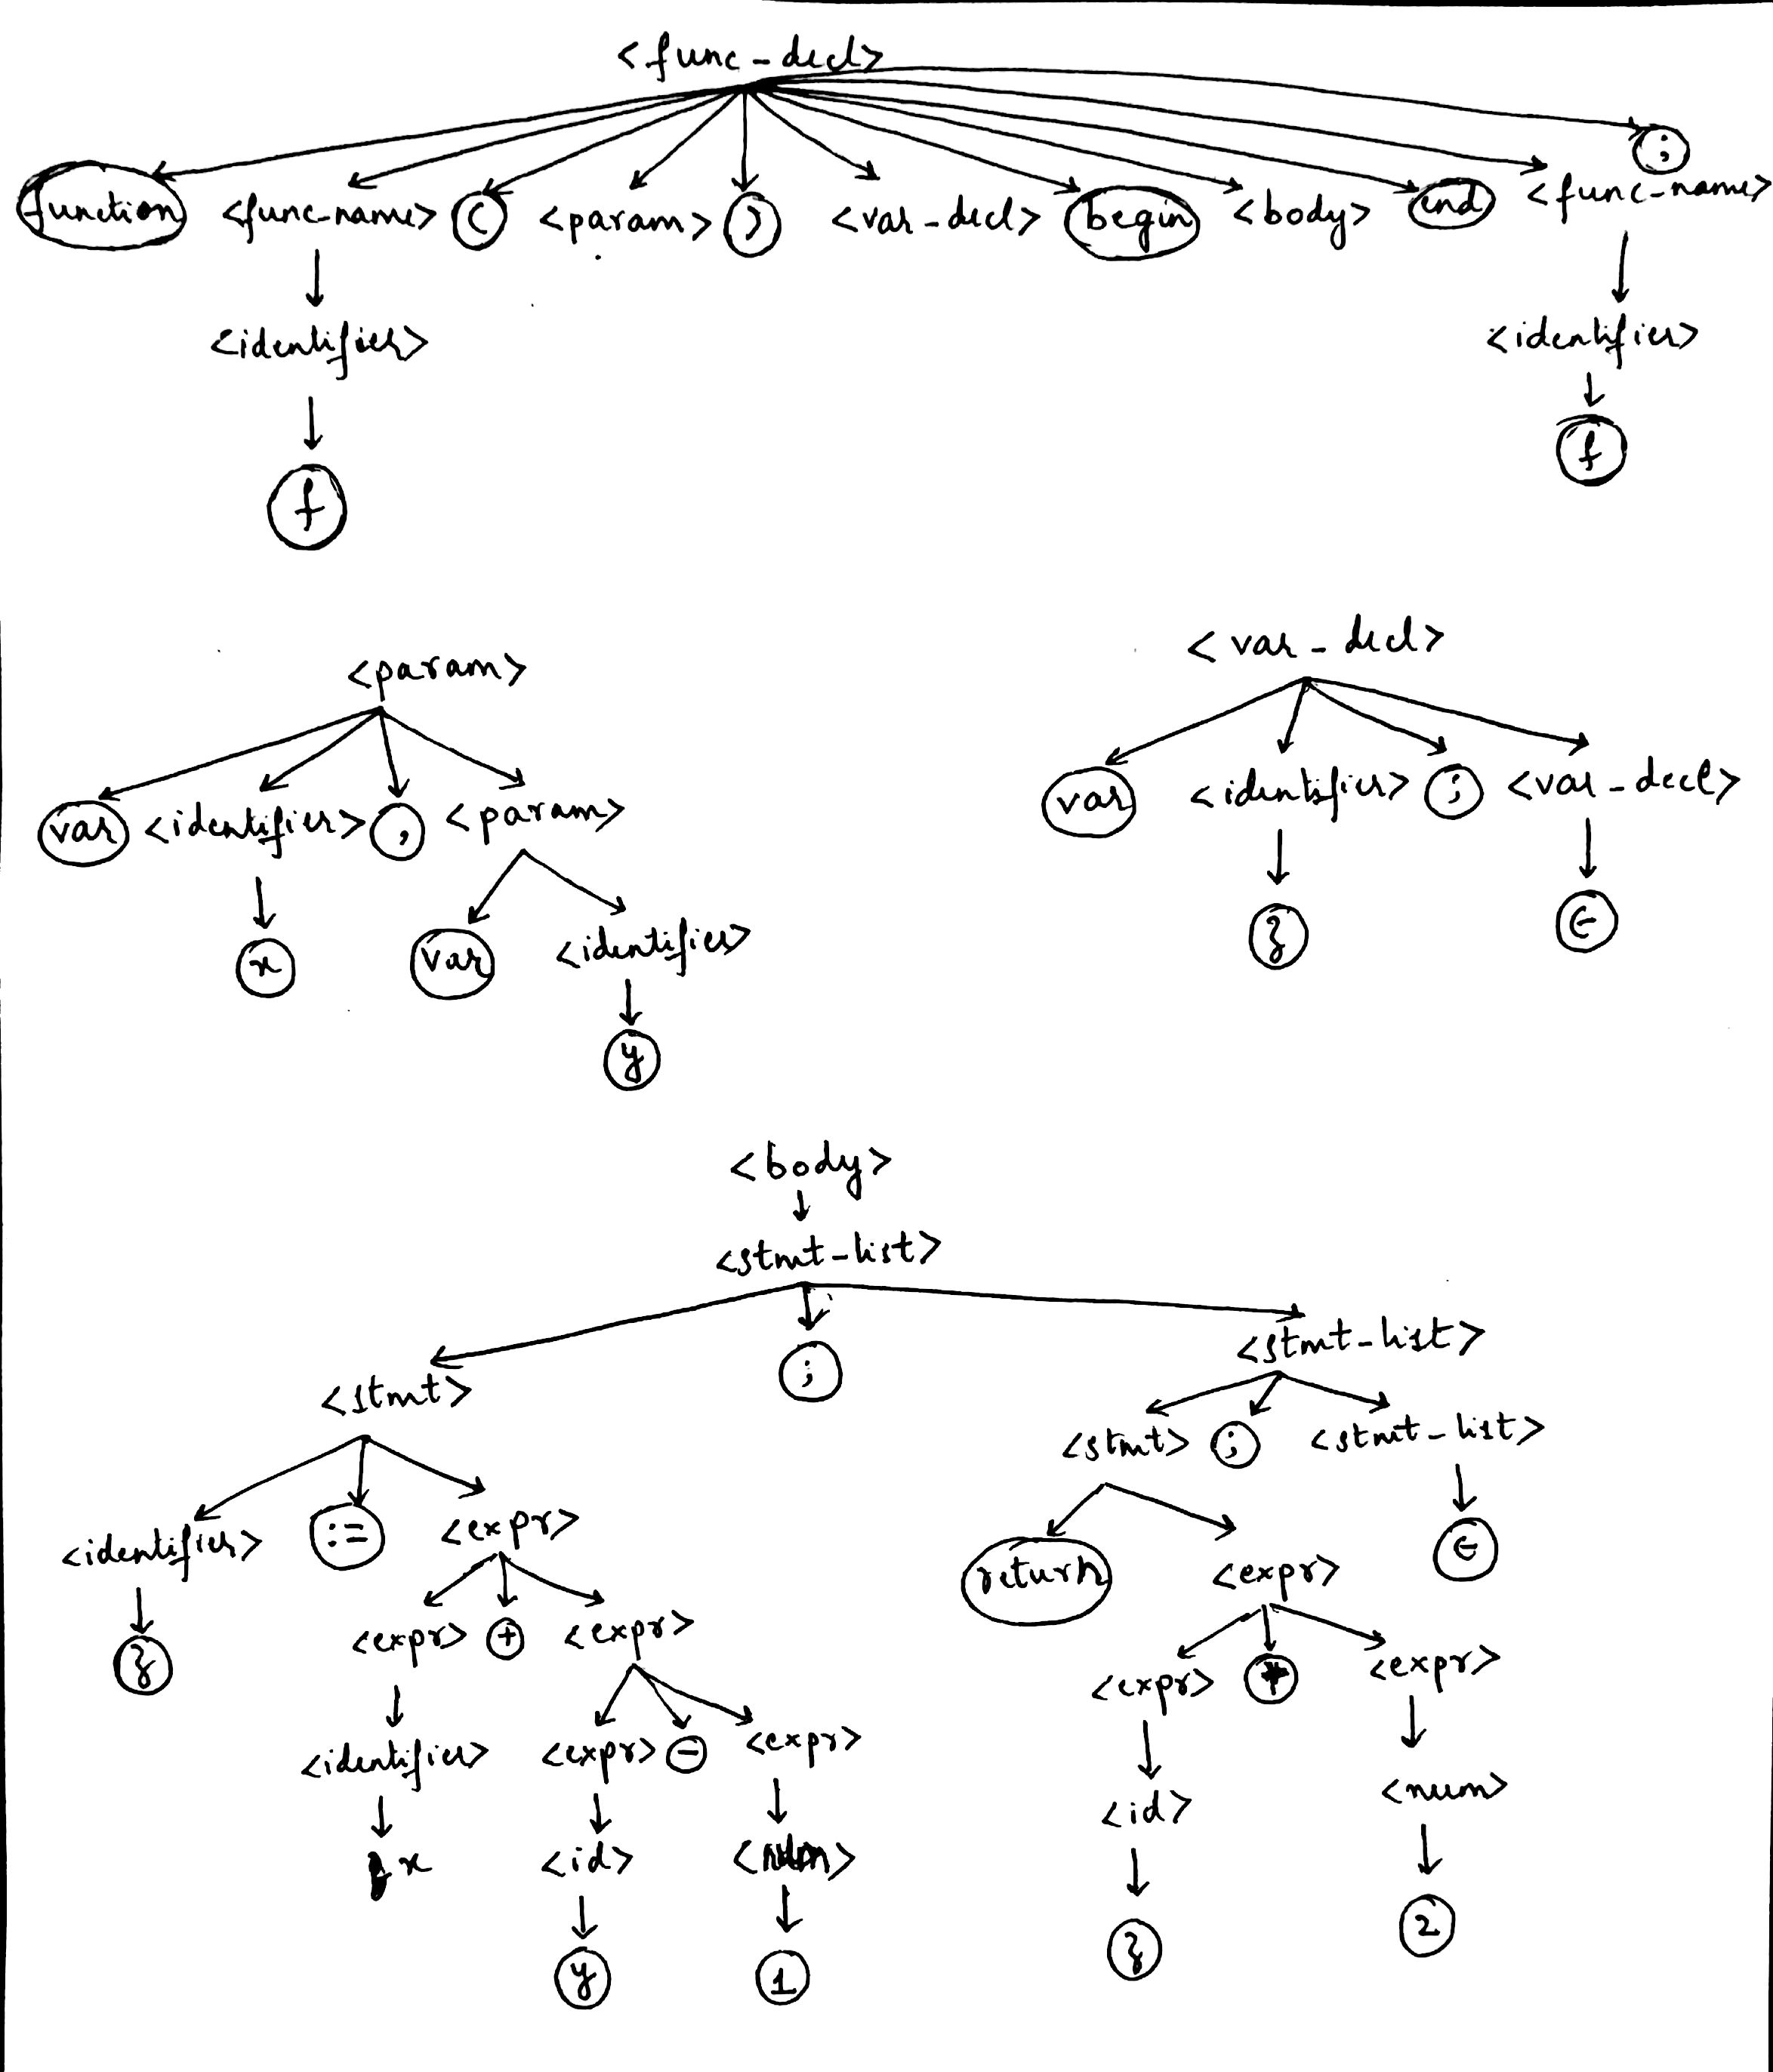
\includegraphics[width=0.95\columnwidth]{f.jpg}
	\caption{Parse tree of function \textit{f}}
	\label{2}
\end{figure}

\begin{figure}[H]
	\centering
	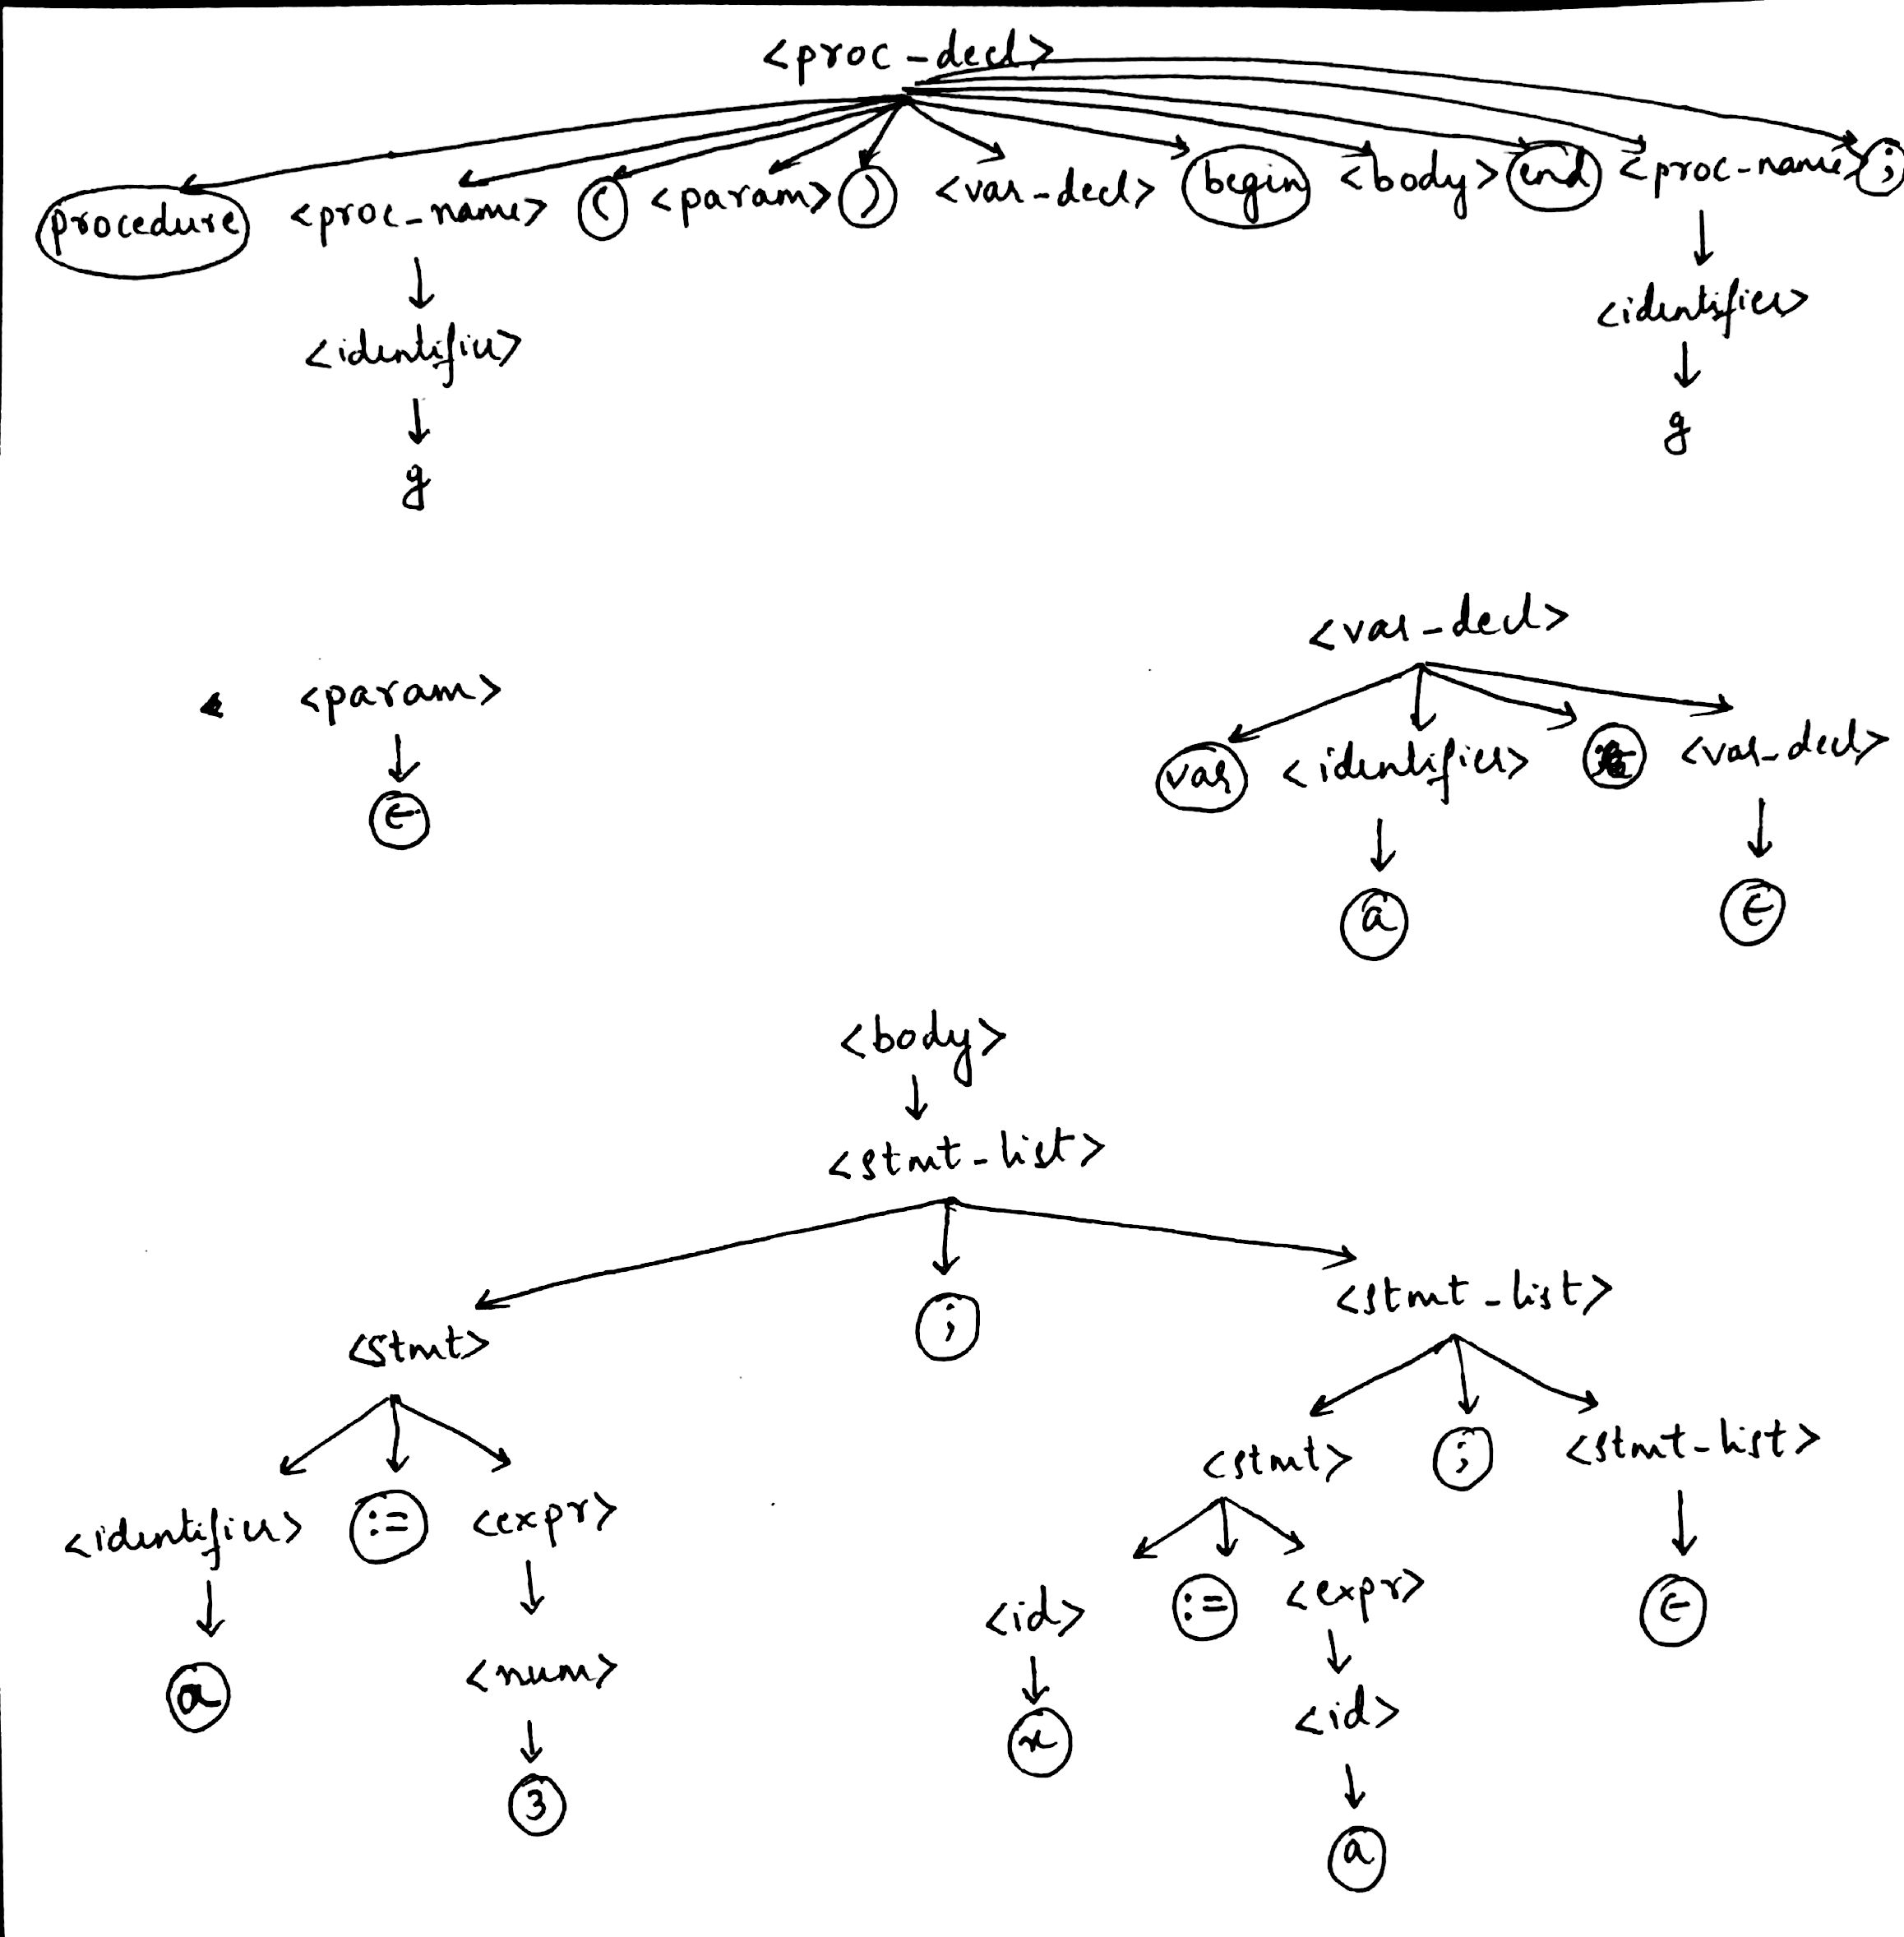
\includegraphics[width=0.95\columnwidth]{g.jpg}
	\caption{Parse tree of procedure \textit{g}}
	\label{3}
\end{figure}
\end{solution}
\fi

\end{itemize}



\newproblem{Polynomial Evaluation}{}

\begin{itemize}

\item[(a)] Define the terms static scoping and dynamic scoping.

\ifnum\me<2
\begin{solution}
\section*{Static Scoping}
In Static scoping, the structure of the program source code determines what variables you are referring to. Therefore the scope of the bindings can be determined at the compile time
\section*{Dynamic Scoping}
In Dynamic scoping, the runtime state of the program stack determines what variable you are referring to. Therefore the scope of the bindings can be determined at the run time
\end{solution}
\fi

\item[(b)] Give a simple example, in any language you like (actual or imaginary), that would
illustrate the difference between static and dynamic scoping. That is, write a short piece
of code whose result would be different depending on whether static or dynamic scoping
was used.

\ifnum\me<2
\begin{solution}
\begin{lstlisting}
program a() {
  x: integer; 
  x = 1;

  procedure b() {
    x = 2;
  }

  procedure c() {
    x: integer;
    b();
  }

  c();
  print x;
}
\end{lstlisting}

With static scoping, we observe the lexical structure of the program source code to see which $x$ we are referring to. There is no definition for $x$ in the local scope for $b$. Hence we look for the definition of $x$ in the statically enclosing scope of $b$ where we can find the global definition of $x$. Therefore this is the $x$ we are referring to in $b$. Therefore $x=2$ writes 2 to the global value of $x$ and 2 will be printed in the case of static scoping

With dynamic scoping, we look for the most active binding made at runtime. So when the program starts running, the global reference to $x$, let it be $x_1$ is pushed onto the stack and then the local definition of $x$ made in $c$ is pushed onto the stack, let it be $x_2$. When $b$ is called from $c$ it looks for the most recent binding of $x$ which is $x_2$. Therefore $x=2$ writes 2 to $x_2$. Now when $c$ returns $x_2$ is popped from the stack and $1$ is printed at the end of the program 
 
\end{solution}
\fi

\item[(c)] In a block structured, statically scoped language, what is the rule for resolving variable
references (i.e. given the use of a variable, how does one find the declaration of that
variable)?

\ifnum\me<2
\begin{solution}
To resolve a reference to any variable, we examine the local scope and statically enclosing scopes until a binding to that variable is found

\end{solution}
\fi

\item[(d)] In a block structured but dynamically scoped language, what would the rule for resolving
variable references be?
\ifnum\me<2
\begin{solution}
To resolve a reference to any variable, we use the most recent, active binding made to that variable at run time

\end{solution}
\fi

\end{itemize}


\newproblem{Asymptotic Comparisons}


\begin{itemize}
\item[(a)]Draw the state of the stack, including all relevant values (e.g. variables, return address,
dynamic link, static link), during the execution of procedure S in the following program.

\begin{lstlisting}
procedure P;
  procedure Q(procedure R)
    procedure S(x:integer);
    begin
      writeln(x);
    end;
  begin (* Q *)
    R(S);
  end;  
  procedure T;
    procedure U(procedure V);
    begin
      V(6);
    end;    
  begin (* T *)
    Q(U);
  end;
begin (* P *)
  T;
end;
\end{lstlisting}

\ifnum\me<2
\begin{solution}

In the below figure, the return address of each stack frame contains the address of the instruction where the function has to return after it's execution
\begin{figure}[H]
	\centering
	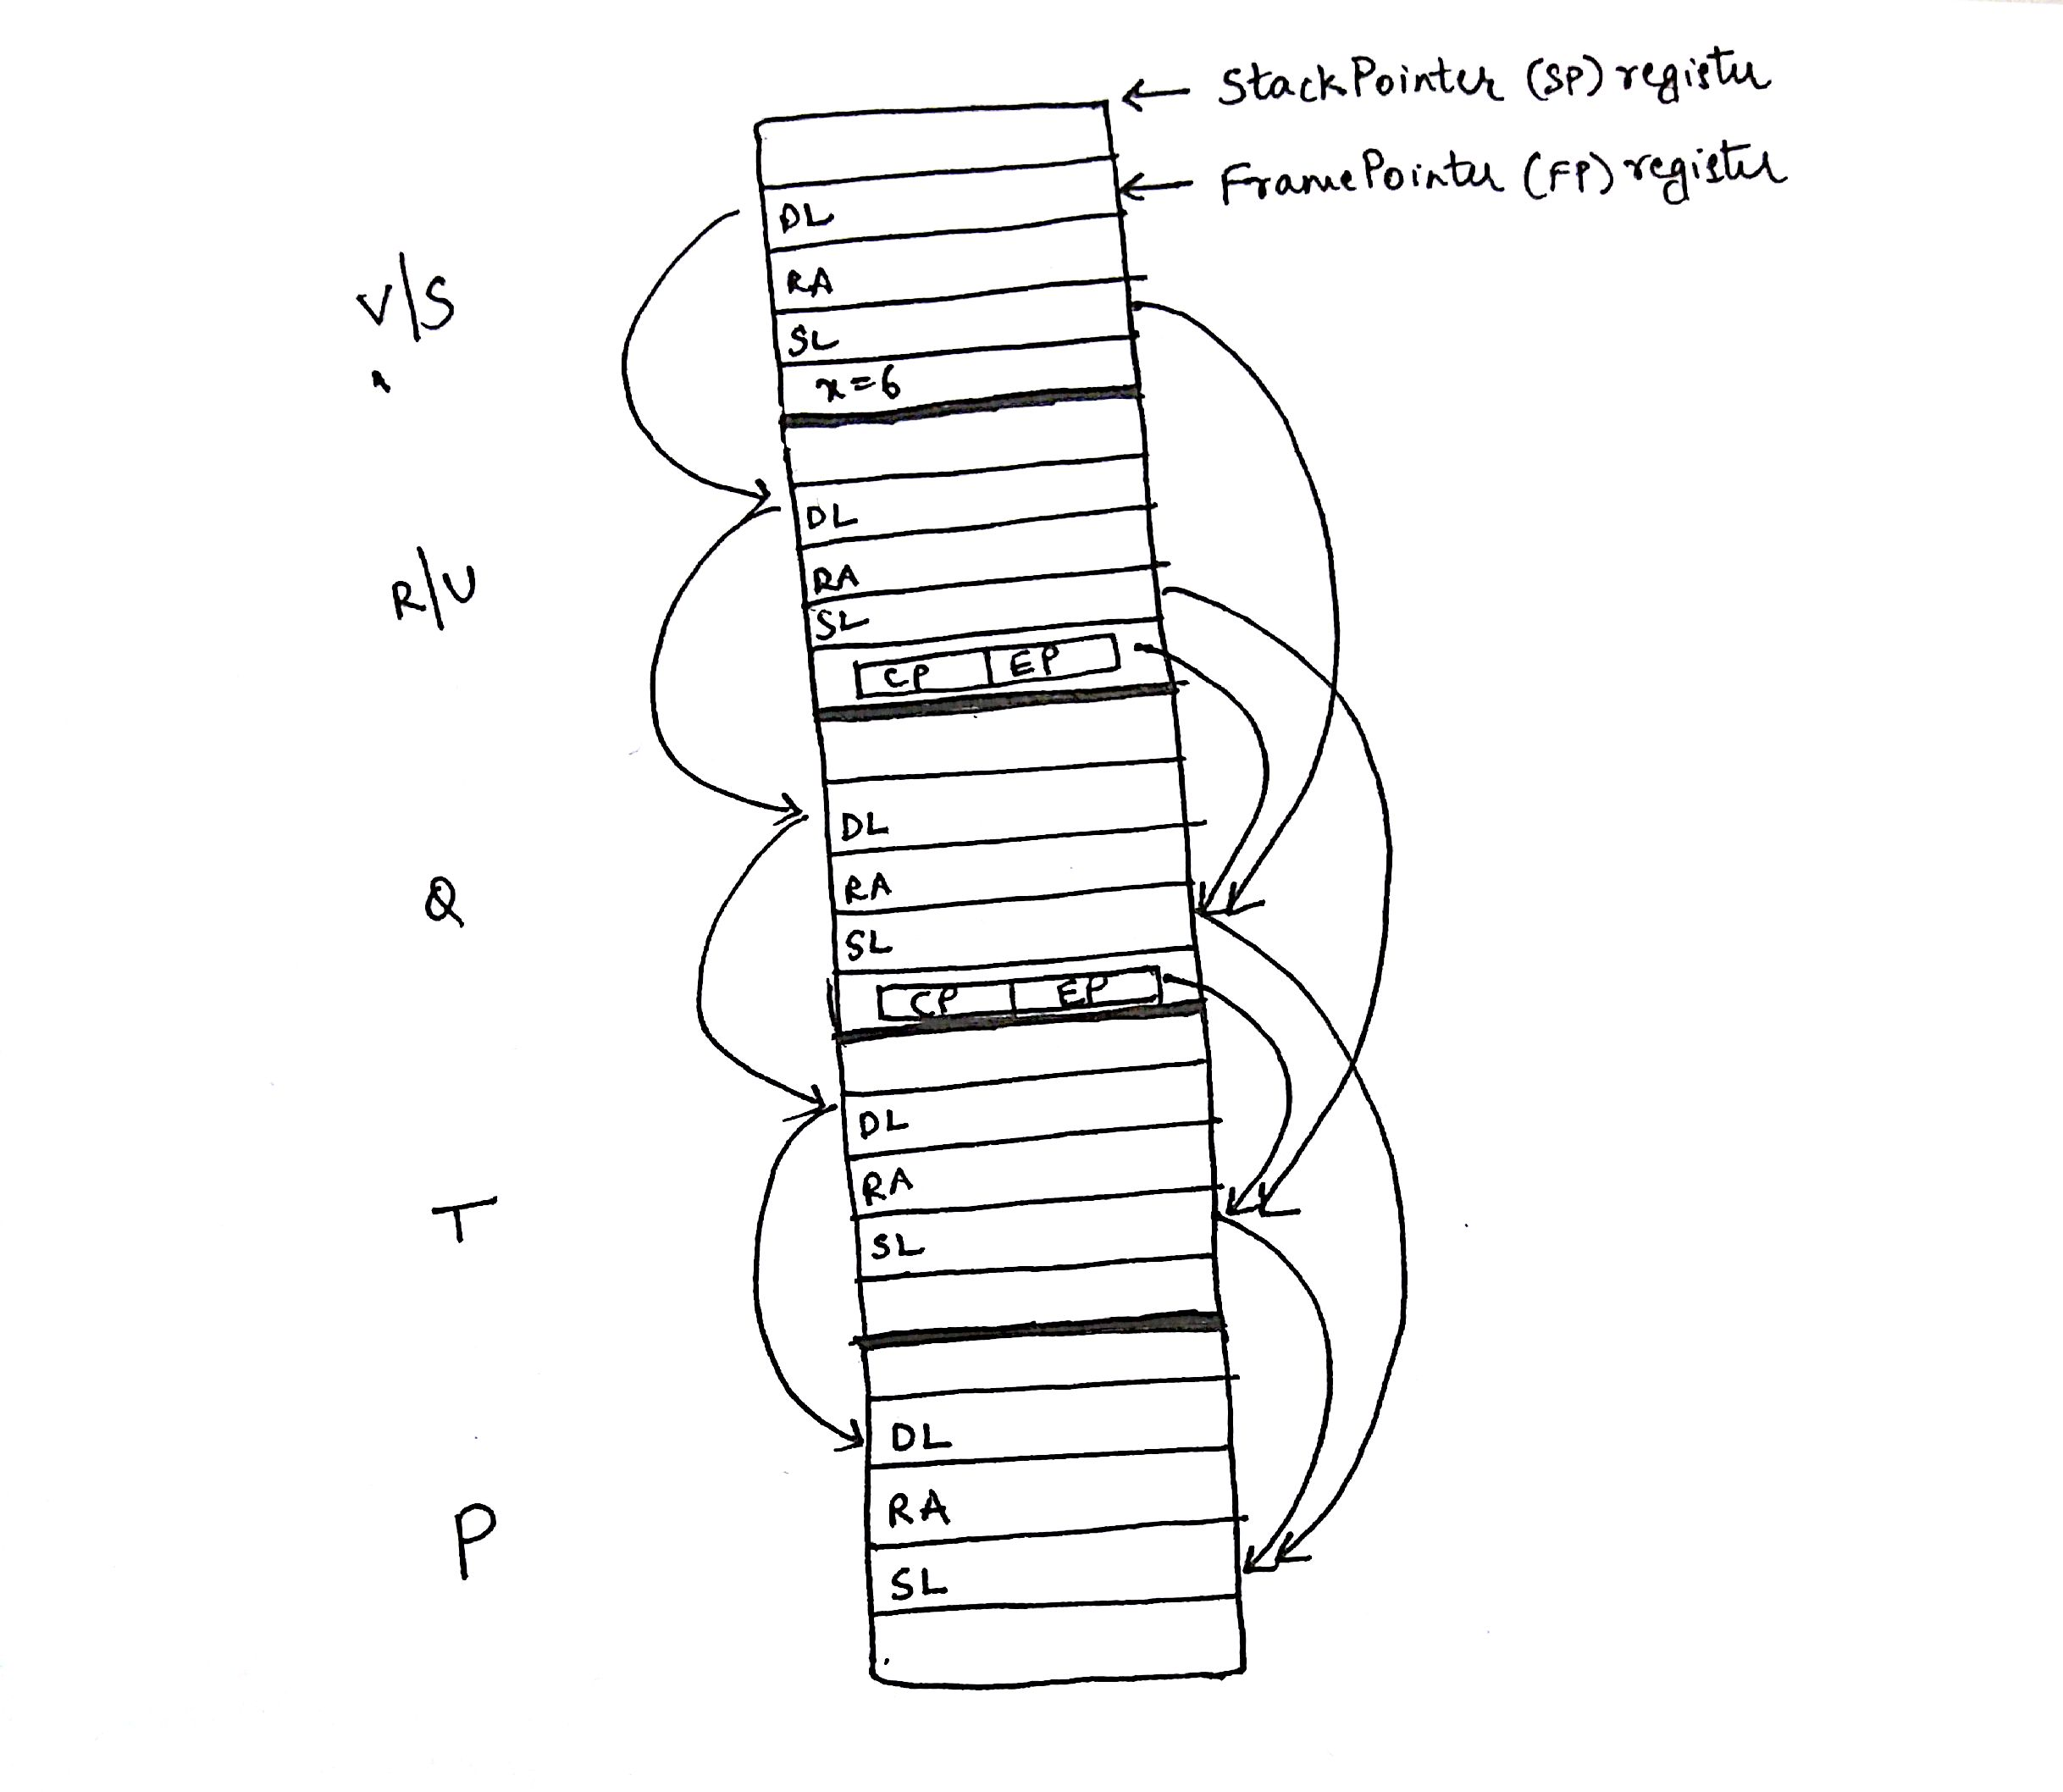
\includegraphics[width=0.95\columnwidth]{callstack.jpg}
	\caption{Call Stack \textit{g}}
	\label{3}
\end{figure}
\end{solution}
\fi
\pagebreak
\item[(b)]Explain why closures on the heap are needed in some languages, and give an example
of a program (in any syntax you like) in which a closure would need to be allocated on
the heap.

\ifnum\me<2
\begin{solution}

Consider the following code, $Q$ is the sub-procedure of $P$ which uses the local variable, $a$ of $P$ and $P$ returns $Q$. 

Therefore, $P$ has to be on top of the stack before calling $Q$ but what if that's not the case. As seen in the code, $T$ calls $P$ and it returns $Q$ into $S$. Now $P$ is popped from the stack and now $S/Q$ is being called. What happens to the $a$ that is being used in $S/Q$ as $P$ is not on the stack anymore

In such a case, we would require to have the closure in the heap and it contains a copy of all the local variables of $P$ that are being used in $Q$
\begin{lstlisting}
procedure P
  a : Integer;
  procedure Q;
  begin
    .....
    a = 5;
  end Q;
begin
  .....
  return Q;
end P;

procedure T
  var S;
begin
  .....
  .....
  S = P();
end T;
\end{lstlisting}
\end{solution}
\fi
\end{itemize}
\newproblem{Asymptotic Comparisons}

For each of these parameter passing mechanisms, state what the following program (in some Pascal-like language) would print if that parameter
passing mechanism was used:

\begin{lstlisting}
program foo;
  var i,j: integer;
  a: array[1..6] of integer;
  procedure f(x,y:integer)
    begin
      x := x * 3;
      i := i + 1;
      y := a[i] + 2;
    end
begin
  for j := 1 to 6 do a[j] = j;
  i := 1;
  f(i,a[i]);
  for j := 1 to 6 do print(a[j]);
end.
\end{lstlisting}


\begin{itemize}
\item[(a)] pass by value
\ifnum\me<2
\begin{solution}

1 2 3 4 5 6
\end{solution}
\fi

\item[(b)]pass by reference

\ifnum\me<2
\begin{solution}

6 2 3 4 5 6
\end{solution}
\fi

\item[(c)] pass by value-result

\ifnum\me<2
\begin{solution}

4 2 3 4 5 6
\end{solution}
\fi

\item[(d)] pass by name

\ifnum\me<2
\begin{solution}

1 2 3 6 5 6
\end{solution}
\fi
\end{itemize}
\newproblem{}

\begin{itemize}
\item[(a)] In Ada, define a procedure containing two tasks, each of which contains a single loop.
The loop in the first task prints the numbers from 1 to 500, the loop in the second task
prints the numbers from 501 to 1000. The execution of the procedure should cause the
tasks to alternate printing fifty numbers at a time, so that the user would be guaranteed
to see:
$1, 2$ $\ldots 50, 501, 502, \ldots, 550, 51, 52, \ldots, 100, 551, 552, \ldots, 600, \ldots$
Be sure there is only one loop in each task.
\ifnum\me<2
\begin{solution}
\begin{lstlisting}
procedure print_1to1000 is
  task print_1to500 is
    entry print;
  end print_1to500;
  task print_501to1000 is
    entry print;
  end print_501to1000;
  
  task body print_1to500 is
  begin
    for i in 1 .. 500 loop
      Put(i);
      if i%50 == 0 then
        print_501to1000.print;
        accept print do
          null;
         end print;
      end if;
    end loop;
    print501_1000.print;
  end print_1to500;
  
  task body print_501to1000 is
  begin
    accept print do
      null;
    end print;
    for i in 501 .. 1000 loop
      Put(i);
      if i%50 == 0 then
        print_1to500.print;
        accept print do
          null;
        end print;
      end if;
    end loop;
  end print_501to1000;
  
begin
  null;
end print_1to1000;
\end{lstlisting}
\end{solution}
\fi

\item[(b)]Looking at the code you wrote for part (a), are the printing of any of the numbers
occurring concurrently? Justify your answer by describing what concurrency is and why
these events do or do not occur concurrently.
\ifnum\me<2
\begin{solution}

Concurrency means that we cannot make any assumptions about the relative ordering of execution of any two or more parts of the code.

But we can clearly see that we are restricting the above code in such a way that the tasks print 1 $\ldots$ 50 51 $\ldots$ 100 $\ldots$ 451 $\ldots$ 500 951 $\ldots$ 1000 by synchronizing the two tasks using the entry calls. Hence there is relative ordering of the execution of the two tasks. Therefore the printing of the numbers is not occurring concurrently
\end{solution}
\fi
\end{itemize}
\end{document}


